\subsection*{Log ind}
Der oprettes en log ind funktion, for at skabe en individuel bruger for den enkelte KOL-patient med henblik på at sikre brugerens private oplysninger samt resultater. Aktivitetsdiagrammet over log ind fremgår af \autoref{fig:logind}. 

\begin{figure} [H]
\centering
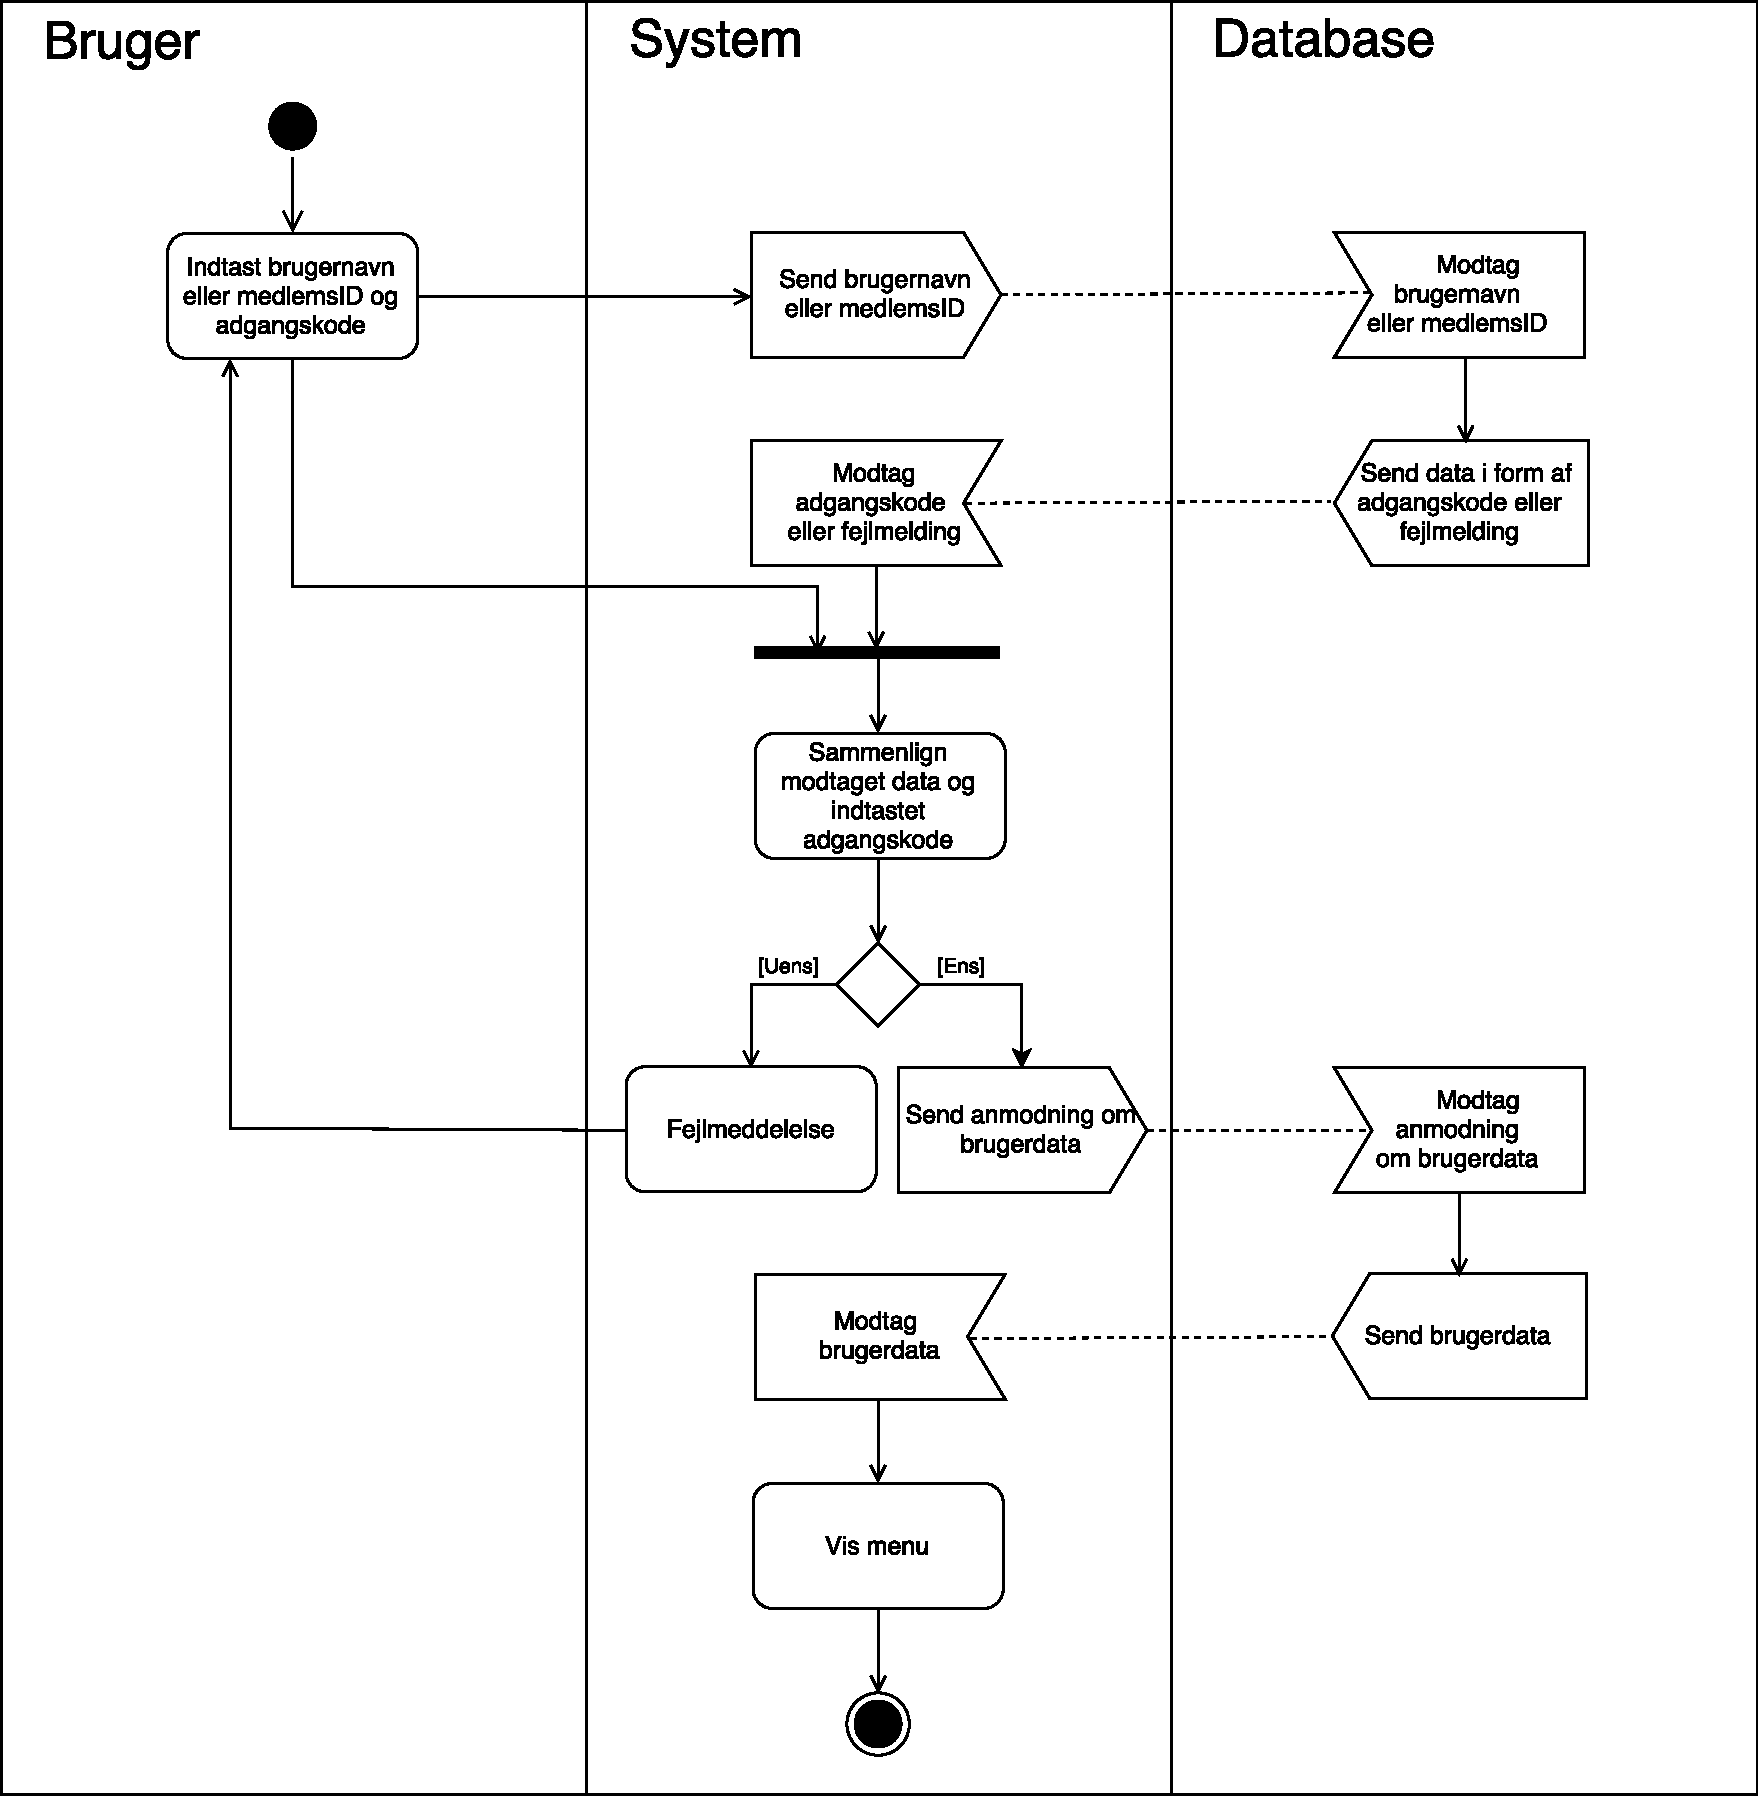
\includegraphics[width=0.9\textwidth]{figures/aktivitetsdiagram/Logind}
\caption{Aktivitetsdiagram over log ind.}
\label{fig:logind}
\end{figure}


\noindent
Når KOL-patienten vil anvende app'en skal medlemsID eller brugernavn samt kodeord indtastes. Systemet sender det indtastede medlemsID eller brugernavn til databasen, som tilbagesender det tilhørende kodeord, hvis det findes i databasen. Hvis de indtastede informationer ikke findes i databasen sendes en fejlmeddelelse i form af 0. Systemet sammenligner herefter brugerens indtastede kodeord med den returnerede værdi fra databasen. Er de to værdier ens, har brugeren indtastet de korrekte informationer, hvortil brugerinformationen hentes fra databasen og hovedmenuen vises. Er de to værdier ikke ens, tilbagesender systemet en fejlmeddelelse og brugeren får derefter mulighed for at indtaste informationer igen. 